\documentclass[12pt]{article}
\usepackage[utf8]{inputenc}


\title{proyecto}
\author{Jose Daniel Rivera }
\date{Julio 2020}
\usepackage[spanish]{babel}

\begin{document}
\title{Proyecto investigacion-hilos. \\}

\maketitle

%\section{}
\noindent
\textbf{¿Qué es una interrupción en el contexto de los microprocesadores?.}
\\
\noindent
\\
Una interrupción es un mecanismo que provoca la alteración del orden lógico de ejecución de instrucciones como respuesta a un evento externo generado por el hardware de entrada/salida en forma asincrónica al programa que está siendo ejecutado y fuera de su control.\\
En forma alternativa se puede decir que una interrupción consiste en un mecanismo que le permite al hardware la invocación de una rutina fuera del control del programa que está siendo ejecutado. \\
\noindent
\\
\textbf{}¿\textbf{Se puede hablar de la historia de las interrupciones?}\\
\noindent
\\
La primera técnica que se empleó para esto fue el polling, que consistía en que el propio procesador se encargará de sondear los dispositivos periféricos cada cierto tiempo para averiguar si tenía pendiente alguna comunicación para él. Este método presentaba el inconveniente de ser muy ineficiente, ya que el procesador consumía constantemente tiempo y recursos en realizar estas instrucciones de sondeo.\cite{elizaldeinterrupciones0}\\
\\
El mecanismo de interrupciones fue la solución que permitió al procesador desentenderse de esta problemática, y delegar en el dispositivo periférico la responsabilidad de comunicarse con él cuando lo necesitara. El procesador, en este caso, no sondea a ningún dispositivo, sino que queda a la espera de que estos le avisen (le "interrumpan") cuando tengan algo que comunicarle (ya sea un evento, una transferencia de información, una condición de error, etc.).
. \cite{lopezfundamentos2010}

\noindent\\
\\
\textbf{¿Que tipo de interrupciones existen?}\\
\\
Las interrupciones se dividen en dos categorías, las de software y las de hardware.
Por sofwtare se encuentra dos ramas: la del sistema y la del usuario, donde la rama del sistema se desglosa en DOS y el ROM BIOS.
Mientras que por el lado del harwdare se divide también en dos ramas: una de ellas es interna y la otra externa, la rama externa se desglosa en dos, en enmascarable y en NO enmascarable.
\\
\noindent
\\
\textbf{¿Cómo se hace la implementación de interrupciones a nivel de hardware?}.\\
\noindent
\\ 
Las interrupciones de hardware son aquellas interrupciones que se producen como resultado de, por lo general, una operación de E/S. No son producidas por ninguna instrucción de un programa sino por las señales que emiten los dispositivos periféricos para indicarle al procesador que necesitan ser atendidos.
Cuando el microprocesador accede a un periférico (disco duro, puerto de comunicación..), puede transcurrir algún tiempo antes de que los datos sean obtenidos o transmitidos. La solución más simple es esperar hasta recibir los datos o hasta que se haya efectuado la transmisión (polling), pero esta solución bloquea todos los programas en ejecución, y eso no puede admitirse en un sistema multitarea. Por ello, en los sistemas modernos se prefiere un funcionamiento mediante interrupciones, ya que éstas permiten mejorar la productividad del procesador, de forma que este último puede ordenar una operación de entrada o salida y, en lugar de tener que realizar una espera activa, se puede dedicar a atender a otro proceso o aplicación hasta que el dispositivo esté de nuevo disponible, siendo dicho dispositivo el encargado de notificar al procesador mediante la línea de interrupción que ya está preparado para continuar o terminar la operación de entrada o salida.\\
\noindent
\\
\textbf{¿Cómo se implementan los hilos por software? Debe quedar claro si el lenguaje de programación importa y si el hardware usado afecta}.\\
\noindent
\\

 Cuando es por hardware se puede realizar a nivel de la CPU (si tiene múltiples entradas de interrupción, ya sean directas o codificadas) ó a nivel del controlador de interrupciones. Cuando es por software el mecanismo se implementa como un algoritmo en la rutina de atención a la interrupción. El algoritmo puede
implementar cualquiera de las estrategias mencionadas, mediante un apropiado recorrido de los controladores de E/S para averiguar cuál fue el que interrumpió, ahora se indicara como puede ser:\\
- recorido lineal: siempre comenzando por el mismo y con un orden preestablecido (prioridad fija)\\
- recorrido programable: utilizando una tabla que establece el orden a seguir (prioridad configurable)\\
- recorrido "round-robin": comenzando cada vez en el siguiente al último
atendido, en forma circular.\cite{aguilerasistemas2015}\\
\\
\textbf{Mostrar un ejemplo de interrupción usando la plataforma Arduino}\\
\\
En el siguiente código definimos el pin digital 10 como salida, para emular una onda cuadrada de periodo 300ms (150ms ON y 150ms OFF).
Para visualizar el funcionamiento de la interrupción,encendemos/apagamos el LED integrado en la placa, por lo que el LED parpadea a intervalos de 600ms (300ms ON y 300ms OFF): No estamos encendiendo el LED con una salida digital, si no que es la interrupción que salta la que enciende y apaga el LED (el pin digital solo emula una señal externa).\\
const int emuPin = 10;\\
const int LEDPin = 13;\\
const int intPin = 2;\\
volatile int state = LOW;\\
void setup() {\\
   pinMode(emuPin, OUTPUT);\\
   pinMode(LEDPin, OUTPUT);\\
   pinMode(intPin, INPUT_PULLUP);\\
   attachInterrupt(digitalPinToInterrupt(intPin), blink, CHANGE);\\
}
void loop() {
   //esta parte es para emular la salida
   
   digitalWrite(emuPin, HIGH);\\
   delay(150);\\
   digitalWrite(emuPin, LOW);\\
   delay(150);\\
}
void blink() {\\
   state = !state;\\
   digitalWrite(LEDPin, state);\\
}
\
\begin{figure}
    \centering
    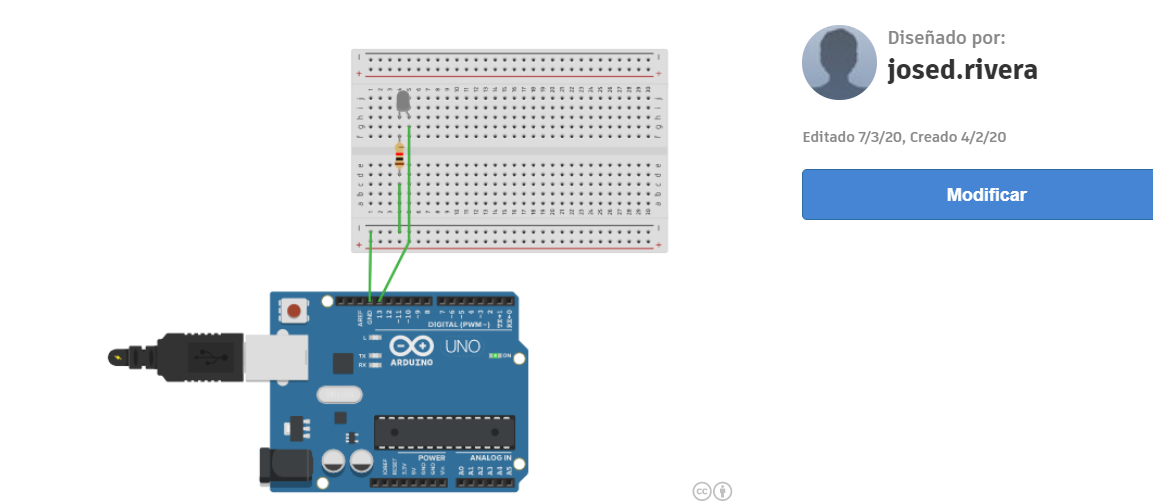
\includegraphics{interrumpcion.png}
    \caption{Caption}
    \label{fig:my_label}
\end{figure}
%\begin{itemize}
    %\item \textbf{}
\bibliographystyle{apalike}
    
\bibliography{referencias}
%\usepackage{natbib}
%\end{itemize}
\end{document}
